\section{Analysis}\label{sec:analysis}
The analysis is divided into three different categories.
However, it should be said at this point that these categories will have overlaps.
Therefore, to avoid mentioning topics several times they will be mentioned only once.
However, this does not rule out that, for example, content from the design category does not also belong to the user or context category.

\subsection{User}
The primary users for this application are persons with mental distress.
The question in this case is: How is mental distress defined, or who is affected by it?
This question gets answered when looking into the core beliefs in the development of Woebot \cite{woebot-beliefs}.

\begin{quote}
    Everybody struggles sometimes. Cognitive distortions are something that everyone experiences in the context of strong emotion; it's part of being human.
\end{quote}

This quote shows clearly that not only persons with strong mental distress should consider using Woebot, but the application is for everyone.
The problem is that design for everyone holds the potential to exclude users by design\cite{feminist-technology}.
Designing for everyone is especially hard, because the human abilities and disabilities are spread in a very wide range.
There are numerous counterexamples for users that do not fall into the extremely broad target group.
Everyone only includes persons being capable of the English language.
And even then it might be hard for persons with dyslexia to communicate with Woebot.\\

\begin{figure}[ht]
    \begin{center}
        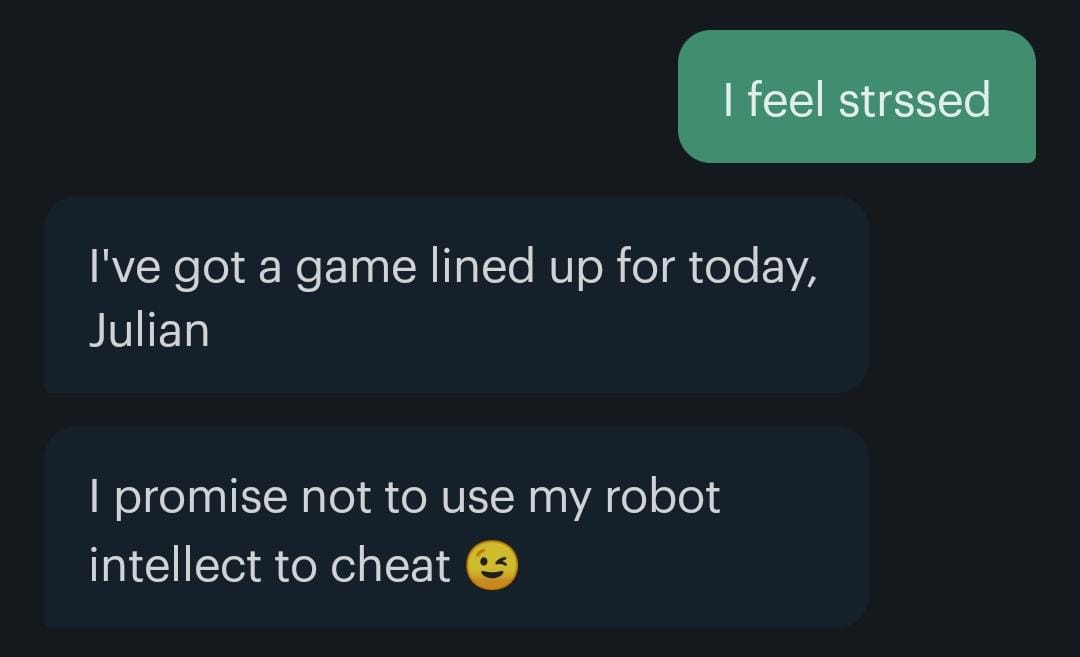
\includegraphics[width=1\columnwidth]{files/dyslexia.png}
        \caption{\label{fig:dyslexia} Cropped screenshot of a misunderstood call for help}
    \end{center}
\end{figure}

\autoref{fig:dyslexia} illustrates the problems that could happen when a typo occurs and Woebot cannot understand the user correctly.
Woebot reacts inappropriate to a user trying to talk about being stressed.
Instead of helping Woebot misunderstands the user and continues suggesting a game, followed up by joking around.
This behavior obviously neglects the feelings of the user.
It has also been observed in a study conducted in 2020\cite{investigating-students}.
Not only did the users feel misunderstood, but the conversations felt repetitive.
Even more problematic is the fact that the user cannot abort the current interaction and is forced to choose one of the predefined answers.\\

The figure also reveals the different problems with NLP, which will be further described in \autoref{sec:design}.
Typos could happen to many target groups.
People with cognitive or motoric disabilities could be affected by this.
A user group that may also not be considered are persons using a dialect of English and therefore be misunderstood.\\

A rather obvious counterexample is the general usage of the application.
It can only be accessed when the people wanting to use the application own a smartphone.
The usage of the application is only limited to a single user.
This can be seen when having a look at the different available lessons.
Although Woebot is capable of suggesting lessons regarding relationships it is not made for usage with more than one user.
However, it could be beneficial for multiple users to attend the proposed lessons together.\\

Woebot cannot only be viewed by the perspective of certain users or a small user group.
The problem of mental health can also be viewed from a societal level.
Here the stigmatization of mental illnesses plays a huge role\cite{stigmatization}.
People are seen as weaker parts of society because of their problems.
Woebot does not fight the stigma but tries to reintegrate people into society as "normal" members.

% GIFs + Emojis - Personal but might be annoying/ not for every target group

\subsection{Design}\label{sec:design}
Woebot is designed as a robot, as the suffix -bot suggests.
The chosen visual design for Woebot seems to be genderless.
This is an interesting design choice, because choosing a gender for a robot can influence human behavior towards the robot.
Researches found out that female voices for example are preferred over male or computer voices\cite{bias-robot}.
Other research has shown that female clients prefer a female therapist and male clients have no preference (58\%), but would rather prefer a female than a male (32\%)\cite{client-gender-preference}.
The reason for preference were among others the feeling of comfort with a female therapist.
Normally such findings would indicate that designing a female conversational agent would lead to a better product.\\

However, a female robot might not only reinforce gender stereotypes, but also reinforce abusive behavior towards the robot\cite{nomura-robot, visual-gender}.
Given the different factors of choosing a gender for a robot, picking a genderless robot seems to be the best solution.
A genderless design does not challenge current gender stereotypes, but it does not reinforce them either.
Woebot is designed with large eyes and a small chin.
This design has been examined and shown that it is perceived as naive, honest, kind and warm\cite{robot-design}.
The perception seems to be similar as the perceived traits of a female therapist, but has to be further examined.\\

Many of Woebot's design problems can be traced back to the first chatbot, ELIZA.
The creator of ELIZA discovered early, that his secretary anthropomorphized the chatbot ELIZA\cite{eliza-chatbot}.
That is not an isolated case, but humans in general tend to anthropomorphize machines.
Computers are social actors (CASA) is the paradigm that describes this phenomenon\cite{casa-first, people-computers}.
This phenomenon can also be transferred to Woebot.
Even if Woebot calls himself a robot, it cannot prevent humans from anthropomorphizing it.
A strong indication for this is a study that shows the therapeutic bond that Woebot is capable of establishing with the user\cite{therapeutic-bond}.
This seems to be a double-edged sword.
The therapeutic bond with the patient ensures that the patient feels more understood.
However, this understanding is only an illusion because Woebot cannot truly understand the user's thoughts.
It could happen that users interpret more knowledge processing into Woebot than it can actually do.\\

Processing user input using NLP is another problem that has accompanied ELIZA's invention.
As shown in \autoref{fig:dyslexia}, Woebot is not able to recognize typos.
In the event of misunderstandings, Woebot reacts with predefined sentences.
However, typos are not the only source of error that occur in a system using NLP.
Misunderstandings can occur for a number of reasons, typos being only one of them.\\

Language is multifaceted and this is exactly where the problem for a text based conversational agent lies.
Phrases can have multiple meanings.
An example for this are homonyms.
Words that have the same spelling but have different meanings.
Semantic ambiguity can also occur in whole sentences.
An example would be: "Call me a doctor".
This could either mean that the person saying this sentence would like to talk to a doctor or would like to be called a doctor.
This ambiguity could be reduced by giving more context.
"I would like you to call a doctor for me" or "Please refer to me as a doctor" would be examples for disambiguation.
Without enough context it is not possible for NLP to process the true meaning of a word or sentence.\\

These problems lie in the design of Woebot.
Due to the chat-like design users might be encouraged to text like they would in a chat with their friends.
Users tend to write without proper punctuation in chat-like services\cite{punctuation}.
The lack of punctuation in instant messaging services are another example for prone to error and lack of context.
The popular example "Let's eat grandpa" and "Let's eat, grandpa" illustrates the problem.
Additionally, an analysis of message length in WhatsApp shows that around 87\% of all messages contain one to ten words\cite{whatsapp-usage}.
The data cannot be transferred completely to Woebot because users may use the application differently than other chat services.
However, the short message length of Woebot and the use of emojis speak for similar results as in the just mentioned study.
According to a psychologist these misunderstandings could have a very negative impact on the user\cite{investigating-students}.

\begin{quote}
    If this happened in therapy, the therapist may lose the client's trust and risk damaging their rapport or therapeutic alliance because it may come across as the therapist ignoring the client's feelings.
    If the client feels unseen/unheard, s/he may not be as receptive to the skills/ lessons available to them in therapy.
\end{quote}

Ready-made answers ensure that the source of error is reduced, but this also ensures that users are forced to give certain answers.
This limitation has the problem that users cannot identify themselves with certain answers\cite{emoticons}.\\

In addition to language-related problems, there are also social and ethical concerns.
Depending on the dataset, linguistic algorithms may contain biased data, which is essentially represented as stereotypical data.
There are many examples of gender bias in NLP as research has shown\cite{gender-bias-nlp}.
Likewise, the origins of bias are also varied\cite{sources-bias-nlp}.\\

When Woebot is first started, a text says that user data is being used to improve the experience.
It also states that data is reviewed anonymously to improve Woebot for everyone.
In addition to that Woebot's privacy police can be found in the settings of the application or online\cite{woebot-privacy}.
First and foremost, it is good that users are made aware of the use of their data.
The problem here is that users may be ignorant of how much information is being shared.\\

Another example of a functionality that is primarily positive but could also turn out to be negative when viewed from a different perspective are the embedded videos.
Take the procrastination lessons for example.
One of the lessons shows the user an informative video about procrastination\cite{procrastination-video}.
The example shows how a person is distracted by movie stars and wants to read more about it online.
After that the person illustrated in the video is distracted by a redirect to a new website.
The new website shows news about a volcano in Indonesia.
The problem here is that the suggested Video from Woebot could lead to the same problem presented in the video.
Since this video is an embedded YouTube video it also suggests other videos to watch at the end.
This could cause users to be lured into continuing to procrastinate just like shown in the video.
An alternative solution would be a video player that does not suggest new videos.\\

There are also several quality of life features that could be implemented.
If you want to look at the chat history to show certain information, for example therapists, there is no way to jump to the newest message using a button.
Another example is the missing description of emojis inside the mood tracker graph shown in \autoref{fig:moodtracker}.
Users might forget what a specific emoji meant and therefore could not fully analyze how they have felt.
Of course the graph shows how positive or negative the mood was, but there is no information about what the emoji represents.
The mood tracker might also be misleading, because the graph always falls back to the baseline after the last tracked mood.
What looks like a prediction on day twelve in \autoref{fig:moodtracker} is actually none.
This could be demotivating to users.
The reason for that is that even if the trend shows that their mood is going into a positive direction the graph always ends up going back to zero.\\

Since many design problems have already been addressed at this point, one last design problem which is questionable will be addressed now.
In order to be able to explain the example, however, a chat history is first shown as an example in which the user has given incorrect information.
The decision-maker lesson teaches the users how to make decisions based on scores that are assigned to tasks.
\autoref{table:chat} shows an excerpt from a conversation with Woebot (W) with the user (U).\\

\begin{table}[ht]
    \begin{tabularx}{\columnwidth}{l X}
        \hline
        Turn & Text                                                                \\
        \hline
        :    &                                                                     \\
        W    & To start, calculate the advantages of option B by adding 100 and 30 \\
        W    & Write it below                                                      \\
        U    & 2                                                                   \\
        W    & Now add the numbers (0+70)                                          \\
        W    & This will be the total disadvantages for option B                   \\
        W    & Write it below                                                      \\
        U    & 1                                                                   \\
        W    & Now to calculate the total for option B, calculate (2-1)            \\
        W    & Notice that minus sign!                                             \\
        W    & Write the result below                                              \\
        U    & 0                                                                   \\
        W    & This number is your total for Option B!                             \\
    \end{tabularx}
    \caption{Excerpt of a conversation with Woebot}
    \label{table:chat}
\end{table}

The miscalculations in \autoref{table:chat} are exaggerated, but illustrate the problem very clearly.
Miscalculations can happen, and it is not okay that incorrect input is used for further calculations.
The idea of giving users a tool that they can use outside Woebot is not a bad thing.
However, in this case, Woebot could have pointed out the miscalculation to the user in a friendly manner.

\subsection{Context}
Changing the context of use of applications can provide further insight into problems.
Especially non-stereotypical contexts highlight weak points of the application.
In this section, two contexts are shown to give examples of different contexts of use.\\

The first context describes an imaginary family that does not have enough money.
Due to the financial situation, the father of the family sinks into a depression.
Since he can't afford therapists, he uses Woebot to learn how to deal with his depression.
The family is also unable to afford multiple smartphones, which is why the children are allowed to use their father's smartphone from time to time.
Mostly to look up things for school or to play mobile games.
Since the father does not want his children to find out about his depression, he sets up a biometric lock in Woebot.
At this point, however, the first problem arises.
The biometric lock can only be set for locking the application after five or thirty minutes.
So it could be that the father uses Woebot and then has to do something urgently while the children have the opportunity to read the sensitive data.\\

\begin{figure}[ht]
    \begin{center}
        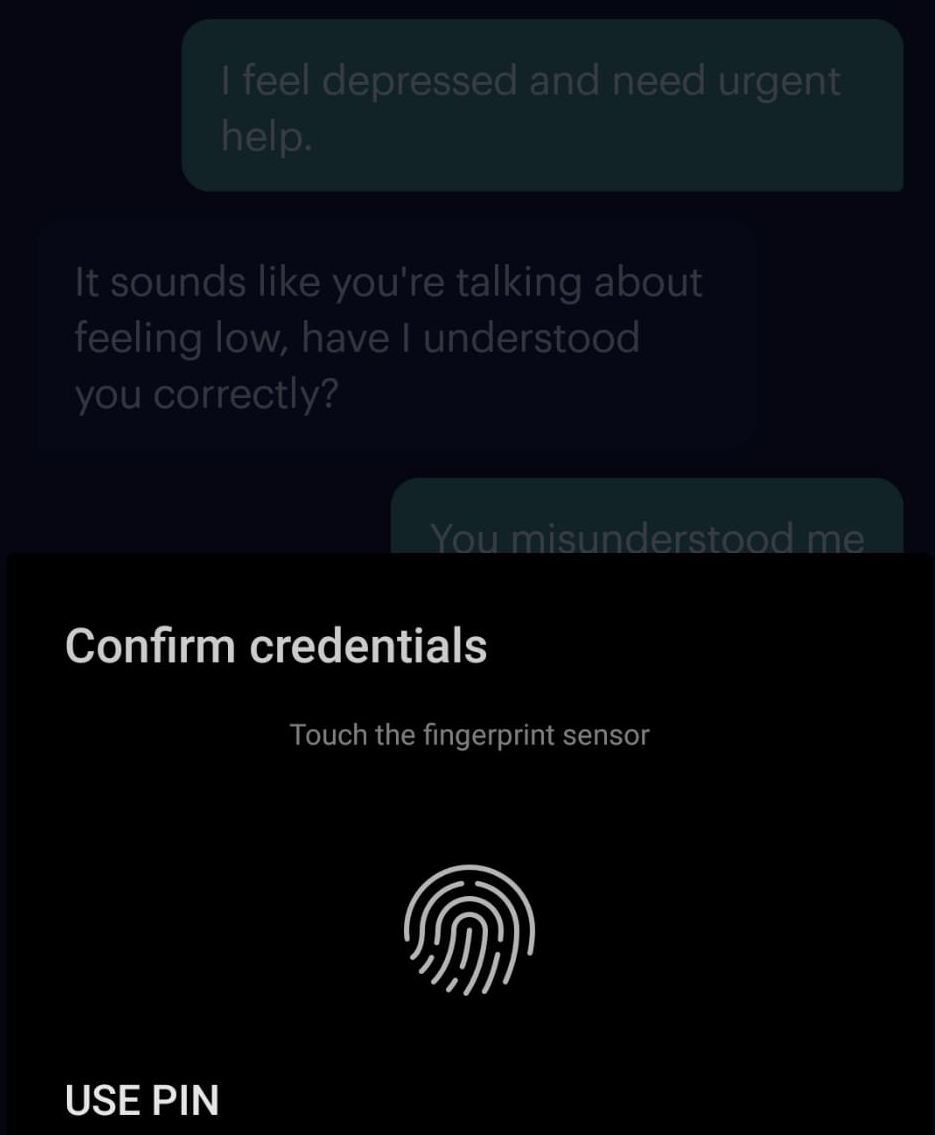
\includegraphics[width=1\columnwidth]{files/biometric-lock.png}
        \caption{\label{fig:biometric-lock} Cropped screenshot of a problem with the biometric lock}
    \end{center}
\end{figure}

However, \autoref{fig:biometric-lock} clearly shows that even with an active biometric lock, the data can be seen clearly.
Content should not be visible before unlocking the application with the biometric lock.\\

The second context refutes a statement made by the founder and president of Woebot Health.
Alison Darcy states\cite{woebot-about}:
\begin{quote}
    Some of our darkest moments happen at 2 AM when there's no one there.
    We designed Woebot to be your personal ally, always available to have a conversation that can help you understand yourself and ease your mind.
\end{quote}
Let us continue with the previously mentioned context with the father of a family.
Due to the lack of money, the father was no longer able to pay for his internet costs.
The problem here is that it is not possible to interact with Woebot without an internet connection.
Neither conversations nor lessons could be started.
It is also not possible to see past moods inside the mood tracker.
Likewise, no messages can be loaded from the gratitude journal.
This refutes Alison Darcy's statement that Woebot is always available.
Of course, the lack of money for an internet connection is not the only problematic context.
Another example would be a girl who has arguments with her parents and withdraws in her room.
The child wants to ask Woebot for help. However, because of the conflict, the parents turned off the Wi-Fi connection on the router.
Therefore, no further interaction with Woebot is possible, and the child is on its own.

%%%%% General TODO %%%%%
% CEO & Founder explanation - Design with actors from the relevant field
